% Options for packages loaded elsewhere
\PassOptionsToPackage{unicode}{hyperref}
\PassOptionsToPackage{hyphens}{url}
\PassOptionsToPackage{dvipsnames,svgnames*,x11names*}{xcolor}
%
\documentclass[
  english,
  man,floatsintext]{apa6}
\usepackage{lmodern}
\usepackage{amsmath}
\usepackage{ifxetex,ifluatex}
\ifnum 0\ifxetex 1\fi\ifluatex 1\fi=0 % if pdftex
  \usepackage[T1]{fontenc}
  \usepackage[utf8]{inputenc}
  \usepackage{textcomp} % provide euro and other symbols
  \usepackage{amssymb}
\else % if luatex or xetex
  \usepackage{unicode-math}
  \defaultfontfeatures{Scale=MatchLowercase}
  \defaultfontfeatures[\rmfamily]{Ligatures=TeX,Scale=1}
\fi
% Use upquote if available, for straight quotes in verbatim environments
\IfFileExists{upquote.sty}{\usepackage{upquote}}{}
\IfFileExists{microtype.sty}{% use microtype if available
  \usepackage[]{microtype}
  \UseMicrotypeSet[protrusion]{basicmath} % disable protrusion for tt fonts
}{}
\makeatletter
\@ifundefined{KOMAClassName}{% if non-KOMA class
  \IfFileExists{parskip.sty}{%
    \usepackage{parskip}
  }{% else
    \setlength{\parindent}{0pt}
    \setlength{\parskip}{6pt plus 2pt minus 1pt}}
}{% if KOMA class
  \KOMAoptions{parskip=half}}
\makeatother
\usepackage{xcolor}
\IfFileExists{xurl.sty}{\usepackage{xurl}}{} % add URL line breaks if available
\IfFileExists{bookmark.sty}{\usepackage{bookmark}}{\usepackage{hyperref}}
\hypersetup{
  pdftitle={Effect of withholding phonetics cues to English-Spanish code-switching},
  pdfauthor={Jiawei Shao},
  pdflang={en-EN},
  pdfkeywords={code-switch, switch cost, reaction time, phonetics, bilingualism},
  colorlinks=true,
  linkcolor=blue,
  filecolor=Maroon,
  citecolor=Blue,
  urlcolor=Blue,
  pdfcreator={LaTeX via pandoc}}
\urlstyle{same} % disable monospaced font for URLs
\usepackage{graphicx}
\makeatletter
\def\maxwidth{\ifdim\Gin@nat@width>\linewidth\linewidth\else\Gin@nat@width\fi}
\def\maxheight{\ifdim\Gin@nat@height>\textheight\textheight\else\Gin@nat@height\fi}
\makeatother
% Scale images if necessary, so that they will not overflow the page
% margins by default, and it is still possible to overwrite the defaults
% using explicit options in \includegraphics[width, height, ...]{}
\setkeys{Gin}{width=\maxwidth,height=\maxheight,keepaspectratio}
% Set default figure placement to htbp
\makeatletter
\def\fps@figure{htbp}
\makeatother
\setlength{\emergencystretch}{3em} % prevent overfull lines
\providecommand{\tightlist}{%
  \setlength{\itemsep}{0pt}\setlength{\parskip}{0pt}}
\setcounter{secnumdepth}{-\maxdimen} % remove section numbering
% Make \paragraph and \subparagraph free-standing
\ifx\paragraph\undefined\else
  \let\oldparagraph\paragraph
  \renewcommand{\paragraph}[1]{\oldparagraph{#1}\mbox{}}
\fi
\ifx\subparagraph\undefined\else
  \let\oldsubparagraph\subparagraph
  \renewcommand{\subparagraph}[1]{\oldsubparagraph{#1}\mbox{}}
\fi
% Manuscript styling
\usepackage{upgreek}
\captionsetup{font=singlespacing,justification=justified}

% Table formatting
\usepackage{longtable}
\usepackage{lscape}
% \usepackage[counterclockwise]{rotating}   % Landscape page setup for large tables
\usepackage{multirow}		% Table styling
\usepackage{tabularx}		% Control Column width
\usepackage[flushleft]{threeparttable}	% Allows for three part tables with a specified notes section
\usepackage{threeparttablex}            % Lets threeparttable work with longtable

% Create new environments so endfloat can handle them
% \newenvironment{ltable}
%   {\begin{landscape}\begin{center}\begin{threeparttable}}
%   {\end{threeparttable}\end{center}\end{landscape}}
\newenvironment{lltable}{\begin{landscape}\begin{center}\begin{ThreePartTable}}{\end{ThreePartTable}\end{center}\end{landscape}}

% Enables adjusting longtable caption width to table width
% Solution found at http://golatex.de/longtable-mit-caption-so-breit-wie-die-tabelle-t15767.html
\makeatletter
\newcommand\LastLTentrywidth{1em}
\newlength\longtablewidth
\setlength{\longtablewidth}{1in}
\newcommand{\getlongtablewidth}{\begingroup \ifcsname LT@\roman{LT@tables}\endcsname \global\longtablewidth=0pt \renewcommand{\LT@entry}[2]{\global\advance\longtablewidth by ##2\relax\gdef\LastLTentrywidth{##2}}\@nameuse{LT@\roman{LT@tables}} \fi \endgroup}

% \setlength{\parindent}{0.5in}
% \setlength{\parskip}{0pt plus 0pt minus 0pt}

% \usepackage{etoolbox}
\makeatletter
\patchcmd{\HyOrg@maketitle}
  {\section{\normalfont\normalsize\abstractname}}
  {\section*{\normalfont\normalsize\abstractname}}
  {}{\typeout{Failed to patch abstract.}}
\patchcmd{\HyOrg@maketitle}
  {\section{\protect\normalfont{\@title}}}
  {\section*{\protect\normalfont{\@title}}}
  {}{\typeout{Failed to patch title.}}
\makeatother
\shorttitle{DS4Ling}
\keywords{code-switch, switch cost, reaction time, phonetics, bilingualism}
\DeclareDelayedFloatFlavor{ThreePartTable}{table}
\DeclareDelayedFloatFlavor{lltable}{table}
\DeclareDelayedFloatFlavor*{longtable}{table}
\makeatletter
\renewcommand{\efloat@iwrite}[1]{\immediate\expandafter\protected@write\csname efloat@post#1\endcsname{}}
\makeatother
\usepackage{csquotes}
\ifxetex
  % Load polyglossia as late as possible: uses bidi with RTL langages (e.g. Hebrew, Arabic)
  \usepackage{polyglossia}
  \setmainlanguage[]{english}
\else
  \usepackage[shorthands=off,main=english]{babel}
\fi
\ifluatex
  \usepackage{selnolig}  % disable illegal ligatures
\fi
\newlength{\cslhangindent}
\setlength{\cslhangindent}{1.5em}
\newlength{\csllabelwidth}
\setlength{\csllabelwidth}{3em}
\newenvironment{CSLReferences}[2] % #1 hanging-ident, #2 entry spacing
 {% don't indent paragraphs
  \setlength{\parindent}{0pt}
  % turn on hanging indent if param 1 is 1
  \ifodd #1 \everypar{\setlength{\hangindent}{\cslhangindent}}\ignorespaces\fi
  % set entry spacing
  \ifnum #2 > 0
  \setlength{\parskip}{#2\baselineskip}
  \fi
 }%
 {}
\usepackage{calc}
\newcommand{\CSLBlock}[1]{#1\hfill\break}
\newcommand{\CSLLeftMargin}[1]{\parbox[t]{\csllabelwidth}{#1}}
\newcommand{\CSLRightInline}[1]{\parbox[t]{\linewidth - \csllabelwidth}{#1}\break}
\newcommand{\CSLIndent}[1]{\hspace{\cslhangindent}#1}

\title{Effect of withholding phonetics cues to English-Spanish code-switching}
\author{Jiawei Shao\textsuperscript{}}
\date{}


\authornote{

The authors made the following contributions. Jiawei Shao: Conceptualization, Writing - Original Draft Preparation, Writing - Review \& Editing.

Correspondence concerning this article should be addressed to Jiawei Shao, Rutgers University. E-mail: \href{mailto:js2845@scarletmail.rutgers.edu}{\nolinkurl{js2845@scarletmail.rutgers.edu}}

}

\affiliation{\phantom{0}}

\abstract{
Code-switching (CS) is the linguistic phenomenon when more than one language is used in one utterance. Various studies have reported switch cost in the recognition, comprehension and production process.

Bilinguals are able to make use of hints in the matrix language of an CS utterance to help themselves recognize and process the upcoming CS phrase.

In this study, we are trying to examine whether Spanish heritage speakers can make use of acoustic cues to mitigate the recognition of upcoming CS items in Enlish-Spanish CS context.

We designed two experiments to test the listeners recognition speed of CS items, one reaction time experiment(listening and pressing button), another eye tracking experiment(listening and choosing corresponding item).

In this paper we'll be focused on the analysis of the first experiment.
}



\begin{document}
\maketitle

\hypertarget{methods}{%
\section{Methods}\label{methods}}

We report how we collect our data, size of sample, all data exclusions (if any), all manipulations, and all measures in the study.

\hypertarget{participants}{%
\subsection{Participants}\label{participants}}

A total of 40 Spanish heritage speakers (20 male, 20 female) were recruited for the present study. All of them are right-handed and showed no speech or hearing defect during the experiment. All participants but one completed both this experiment and Experiment 2. When recruiting, all of them self-reported as intermediate-advanced level Spanish speaker who have at least the level of B2 under DELE scheme. Each of the participants finished an adapted language history questionnaire based on LHQ3 (Li, Zhang, Yu, \& Zhao, 2020), an adapted DELE exam testing their reading comprehension, grammar, listening comprehension and speaking skills, and an adapted BSWQ (Rodriguez-Fornells, Kramer, Lorenzo-Seva, Festman, \& Münte, 2012) after the two experiments. The language proficiency test result shows that all the participants are as fluent as their claim when being recruited in comprehension and speaking tests, while 2 of them had a beginner-intermediate level of proficiency for grammar test. The participants all live in the same community where the most commonly used variate of Spanish is Mexican Spanish, they are all born in Mexico and moved to the US with their entire family before age of 8, and have been living in the US for at least 15 years. The average age was 20.4 years (SD = 2.2). All participants reported regularly code-switching with friends or family. The participants' language dominance is evaluated by Bilingual Language Profile (Birdsong, Gartken, \& Amengual, 2012) integrated in the LHQ3. The qualitative questions shows that all the participants tend to speak in Spanish within their families and English is more dominant in working and studying environments. The Bilingual Language Profile result shows that, they are all English dominant. BSWQ result shows that they are frequent code switchers that equally switch in either of the directions. The family and community they live in also is reported to be an environment where CS regularly happens. The language background information of the particianps is presented in Table 1.

\begin{table}[tbp]

\begin{center}
\begin{threeparttable}

\caption{\label{tab:data participants}Language information of the participants}

\begin{tabular}{llllll}
\toprule
sub\_partcipants\_condition & \multicolumn{1}{c}{n} & \multicolumn{1}{c}{Mean} & \multicolumn{1}{c}{SD} & \multicolumn{1}{c}{Min} & \multicolumn{1}{c}{Max}\\
\midrule
age & 40 & 20.30 & 1.96 & 15.45 & 24.20\\
age\_acq & 40 & 4.18 & 2.72 & 0.11 & 10.85\\
CSF & 40 & 5.82 & 0.82 & 3.37 & 7.40\\
EN\_ES & 40 & 6.09 & 0.40 & 5.29 & 6.90\\
LP & 40 & 5.23 & 0.66 & 3.63 & 6.60\\
\bottomrule
\addlinespace
\end{tabular}

\begin{tablenotes}[para]
\normalsize{\textit{Note.} age:age of the participant; age\_acq: age of acquisition of English; CSF: code-switching frequency, EN\_ES: use of either languages with family and friends, 0 means always in English, 7 means always in Spanish; LP:language proficiency in Spanish.}
\end{tablenotes}

\end{threeparttable}
\end{center}

\end{table}

\hypertarget{material-and-procedure}{%
\subsection{Material and Procedure}\label{material-and-procedure}}

The current study adopts splicing manipulation to make stimulus to test the predictions. When preparing auditory materials, we spliced for both experiments: we spliced Spanish code-switched items from English-Spanish code-switched sentences (e.g., When I was reading a book under the tree, una manzana se cayó en mi cabeza.) into English sentences that were originally unilingual (e.g., When I was reading a book under the tree, an apple fell on my head.) to withhold any anticipatory phonetic cues to the code-switch. By doing so, bias will be created that the listeners may not be excepting the utterance that started in English will suddenly switch to Spanish, as all the potential acoustic cue were eliminated from the matrix language. We then will compare, respectively in experiment 1 and experiment 2, the reaction time to press the button indicating the recognition of the visual stimuli in the recording, and fixation time on the target item. We prepared four conditions for analysis: unilingual unspliced, CS unspliced, CS spliced and CS spliced control .Figure 1 shows the different conditions of the stimulus.

\begin{figure}

{\centering 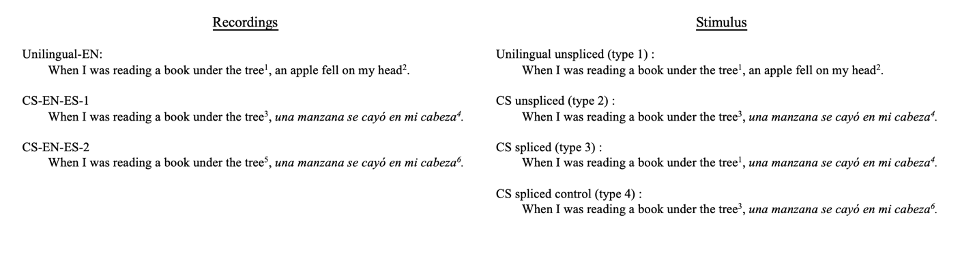
\includegraphics[width=9.05in]{figure/figure_conditions_stimuli} 

}

\caption{conditions of stimulus}(\#fig:conditioins of stimulus)
\end{figure}

Data collection took place in a sound-attenuated booth. During the experiments, participants saw a picture in the center of the computer screen, and as the audio being played, listeners should press a button as soon as they heard the object mentioned in the sentence. The software was programmed as when a sentence contains a noun that paired with the picture and in 3000 ms the participant still does not have any reaction, it will be skipped automatically. Reaction time is being recorded automatically. Figure 2 shows the procedure of experiment 1.

\begin{figure}

{\centering 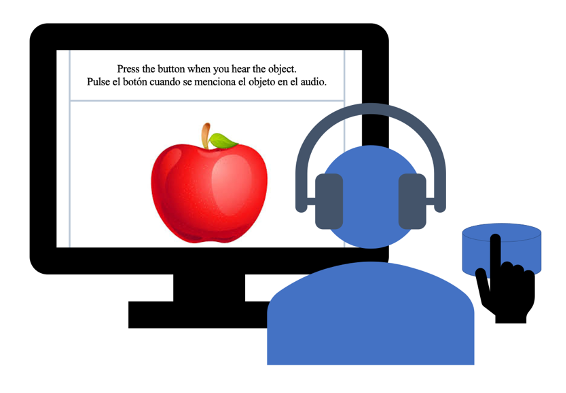
\includegraphics[width=11.32in]{figure/figure_setting} 

}

\caption{experiment setting}\label{fig:setting}
\end{figure}

\hypertarget{results-and-analysis}{%
\section{Results and analysis}\label{results-and-analysis}}

The RT data from experiment 1 were collected and stored by group of type of stimulus. We then submitted the data to four analyses. The objective of the first analysis was to get an overall understanding of the relation between type of stimulus and reaction time. To this end, we tidied up the data. Based on the tidy data we made one table and one plot. The purpose of the first analysis is to determine if the results are consistant with our prediction that listeners can make use of phonetic cues to cope with switch cost(RT type 2 should be longer than RT type 1), and by splicing the RT will be longer because of the absence of the phonetic cues(RT type 3 should be longer than type 2), while the splicing process itself won't make any difference (RT type 2 should be similar to type 4). The result are presented in Table 2 and Figure 3. As the distribution of Figure 3 suggests, that in both conditions of the experiments, type 1 stimuli have the shortest RT(mean = 708.8, SD = 86.57), type 2 and type 4 are close(mean(type2) = 857.1, SD(type2) = 85.39, mean(type4) = 858.0, SD(type4) = 84.72), and the spliced type 3 shows longest RT(mean = 918.4, SD = 86.11).

\begin{table}[tbp]

\begin{center}
\begin{threeparttable}

\caption{\label{tab:table3}Summerized results of experiment 1}

\begin{tabular}{lllll}
\toprule
stim\_version & \multicolumn{1}{c}{Mean} & \multicolumn{1}{c}{SD} & \multicolumn{1}{c}{Min} & \multicolumn{1}{c}{Max}\\
\midrule
type1 & 741.24 & 87.20 & 533.03 & 949.74\\
type2 & 891.21 & 86.87 & 681.16 & 1,100.39\\
type3 & 949.86 & 87.49 & 754.49 & 1,159.57\\
type4 & 891.03 & 88.57 & 671.94 & 1,119.04\\
\bottomrule
\addlinespace
\end{tabular}

\begin{tablenotes}[para]
\normalsize{\textit{Note.} RT unit = ms}
\end{tablenotes}

\end{threeparttable}
\end{center}

\end{table}

\begin{figure}
\centering
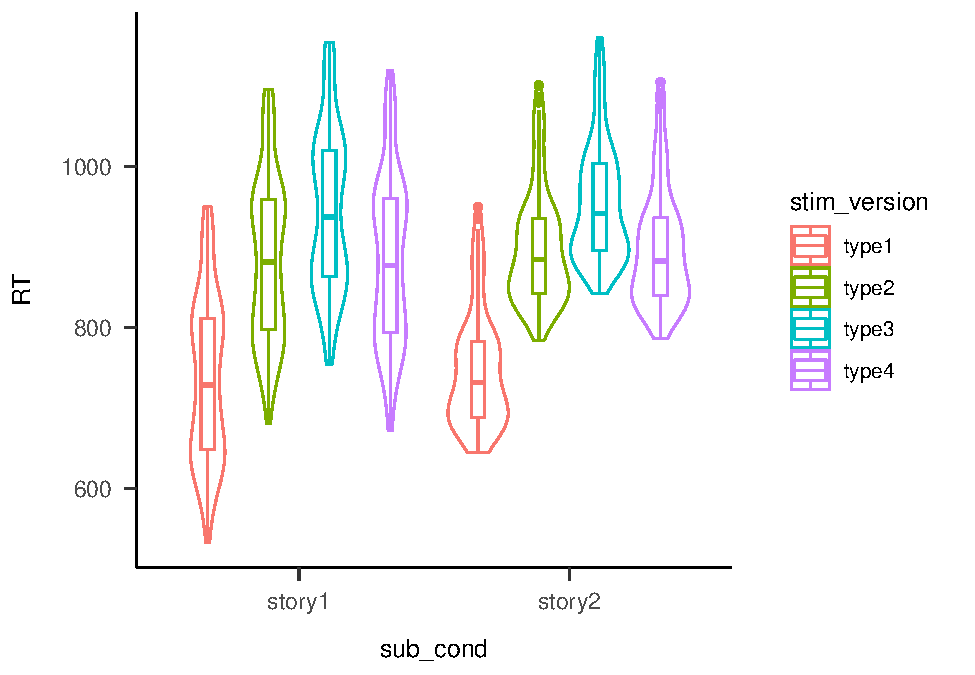
\includegraphics{FP_Jiawei_files/figure-latex/plot1-1.pdf}
\caption{\label{fig:plot1}Median search time}
\end{figure}

The second analysis of the data examined RT and the correlation with the type of stimuli. The second analysis focus on the comparison of type 1 and type 2, which are naturally produced unilingual English sentences and naturally produced CS sentences. The purpose of this analysis is to determine the effect of switch cost in a naturalistic setting. The data were analyzed using generalized linear mixed effects models (GLMM). The categorical fixed effect group was dummy coded with type 1 set as the baseline. The random effects structure included by-subject and random intercepts and random slopes.

The GLMM was best fit when including the random effects. There was a main effect of type of stimuli(type 1 vs type 2). For the type 2 group the RT were longer by 149.97 ± 1.35 se (t=111.1, p\textless0.001).

The third analysis of the data examined RT and the correlation with the type of stimuli focusing on the comparison of type 2 and type 4, which are naturally produced CS sentences and spliced CS sentences yet still maintianing phonetic cues. The purpose of this analysis is to determine the whether the process of splicing can cause effect for RT. The data were analyzed using generalized linear mixed effects models (GLMM). The categorical fixed effect group was dummy coded with type 2 set as the baseline. The random effects structure included by-subject and random intercepts and random slopes.

The GLMM was best fit when including the random effects. There wasn't a main effect of type of stimuli(type 2 vs type 4), for the type 4 group the RT were shorter by 0.178 ± 1.397 se (t=-0.13, p=0.9).

The forth analysis of the data examined RT and the correlation with the type of stimuli focusing on the comparison of type 2 and type 3, which are naturally produced CS sentences and spliced CS sentences without phonetic cues. The purpose of this analysis is to determine the whether eliminating phonetic cues in matrix lanugage can cause longer RT. The data were analyzed using generalized linear mixed effects models (GLMM). The categorical fixed effect group was dummy coded with type 2 set as the baseline. The random effects structure included by-subject and random intercepts and random slopes.

The GLMM was best fit when including the random effects. There wasn a main effect of type of stimuli(type 2 vs type 3), for the type 3 group the RT were longer by 58.65 ± 1.47 se (t=40, p\textless0.001).

\hypertarget{discussion-and-conclusion}{%
\section{Discussion and conclusion}\label{discussion-and-conclusion}}

As we predict, the RT of type 1 and type 2 show significant difference, as the in comparison with RT-type-1, the type 2 are naturally produced CS sentences that can cause switch cost for the listeners when comprehending. It confirms the premise of the experiment that the switch cost for the participants aren't caused by accident.
RT-type-2 and RT-type-4 didn't show significant difference as the type 4 sentences were created using splicing without eliminating the phonetic cues. This step confirms that the splicing process itself won't be a irrelevant variable. By splicing, the only variable changed is the whether the phonetic cues are in the sentence.
RT-type-2 and RT-type-3 shows a significant difference, yet the difference is smaller in quantatively comparing to type 1 vs type 2. The RT-type-4 will be longer than RT-type-2 as the phonetic cues were absent. This suggest that the existence of phonetic cues could be helpful for listners to recognize CS items. This can also suggest a predictive role of the phonetic cues.

\newpage

\hypertarget{references}{%
\section{References}\label{references}}

\begingroup
\setlength{\parindent}{-0.5in}
\setlength{\leftskip}{0.5in}

\hypertarget{refs}{}
\begin{CSLReferences}{1}{0}
\leavevmode\hypertarget{ref-bir2012}{}%
Birdsong, D., Gartken, L. M., \& Amengual, M. (2012). Bilingual language profile: An easy-to-use instrument to assess bilingualism. \emph{Bilingual Language Profile}. COERLL, University of Texas at Austin. Retrieved from \url{https://sites.la.utexas.edu/bilingual/}

\leavevmode\hypertarget{ref-li2020}{}%
Li, P., Zhang, F., Yu, A., \& Zhao, X. (2020). Language history questionnaire (LHQ3): An enhanced tool for assessing multilingual experience. \emph{Bilingualism: Language and Cognition}, \emph{23}(5), 938--944.

\leavevmode\hypertarget{ref-li2020}{}%
Li, P., Zhang, F., Yu, A., \& Zhao, X. (2020). Language history questionnaire (LHQ3): An enhanced tool for assessing multilingual experience. \emph{Bilingualism: Language and Cognition}, \emph{23}(5), 938--944.

\leavevmode\hypertarget{ref-rod2012}{}%
Rodriguez-Fornells, A., Kramer, U., Lorenzo-Seva, U., Festman, J., \& Münte, T. (2012). Self-assessment of individual differences in language switching. \emph{Frontiers in Psychology}, \emph{2}, 388. \url{https://doi.org/10.3389/fpsyg.2011.00388}

\end{CSLReferences}

\endgroup


\end{document}
